In \Cref{sec:methods}, we describe the problem setup of dimensionality reduction for document retrieval.
We discuss the results of different compression methods (random projections, PCA, autoencoder, precision reduction and their combination) in \Cref{sec:model_comparison} and provide further analysis in \Cref{sec:analysis}.

\section{Problem Statement} \label{sec:methods}

To speed up the similarity computation over a large set of documents and to decrease memory usage ($f_D$ is usually precomputed), we apply \textbf{dimension reduction functions} $r_Q : \mathbb{R}^d \rightarrow \mathbb{R}^{d'}$ and $r_D : \mathbb{R}^d \rightarrow \mathbb{R}^{d'}$ for the query and document embeddings respectively. Formally, we are solving the following problem (extended from \Cref{sec:intro_setup}):
\begin{align}
Z &= \argk_{d \in \mathcal{D}}~ \text{rel.}(q, d)~, \text{with}\\
\text{rel.}(q, d) &\approx \text{sim}(f_\text{Q}(q), f_\text{D}(d)) \\
&\approx \text{sim}(r_\text{Q}(f_\text{Q}(q)), r_\text{D}(f_\text{D}(d)))
\end{align}

Since $f_Q$ is commonly fine-tuned for a specific downstream task, it is desirable in (3) for the functions $r_Q$ and $r_D$ to be differentiable so that they can propagate the signal.
These dimension-reducing functions need not be the same because even though they project to a shared vector space, the input distribution may still be different.
Similarly to the query and document embedding functions, they can be fine-tuned.

\subsection{Pre-processing Transformations}

\Cref{fig:model_intro} also shows that model performance, especially for DPR, depends heavily on what similarity metric is used for retrieval.
This is because none of the models produces normalized vectors by default.

\Cref{fig:model_normalization} shows that performing only normalization $\big(\frac{\bm{x}}{||\bm{x}||}\big)$ sometimes hurts the performance but when joined with centering beforehand $\big(\frac{\bm{x}-\bar{\bm{x}}}{||\bm{x}-\bar{\bm{x}}||}\big)$, it improves the results (compared to no pre-processing) in all cases.
The normalization and centering is done for queries and documents separatedly.
Moreover, if the vectors are normalized, then the retrieved documents are the same for $L^2$ and inner product.
\footnote{$
\argmax_k -||\bm{a}-\bm{b}||^2 =
\argmax_k -\langle \bm{a},\bm{a} \rangle^2 - \langle \bm{b},\bm{b} \rangle^2 + 2\cdot \langle \bm{a},\bm{b} \rangle =
\argmax_k\ 2\cdot \langle \bm{a},\bm{b} \rangle - 2 = \argmax_k\ \langle \bm{a},\bm{b} \rangle$}

Nevertheless, we argue it still makes sense to study the compression capabilities of $L^2$ and the inner product separately, since the output of the compression of normalized vectors need not be normalized.

Another common approach before any feature selection is to use z-scores ($\frac{x-\bar{x}}{\sigma}$) instead of the original values.
Its boost in performance is however similar to that of centering and normalization.
The effects of each pre-processing step are in \Cref{tab:zscore}.
The significant differences in performance show the importance of data pre-processing (agnostic to model selection).

\begin{table}[ht]
\center
\begin{tabular}{lcccc}
    \toprule
     & \textbf{IP} & $\mathbf{L^2}$ \\
    \midrule
    DPR-CLS & $0.609$ & $0.240$ \\
    \cmidrule{1-3}
    Center & $0.630$ & $0.353$ \\
    Z-Score & $0.632$ & $0.525$ \\
    Norm. & \multicolumn{2}{c}{$0.463$} \\
    Center + norm. & \multicolumn{2}{c}{$0.618$} \\
    Z-Score + norm. & \multicolumn{2}{c}{$0.621$} \\
    % BIG-HP
    % - & $0.427$ & $0.092$ \\
    % Center & $0.414$ & $0.201$ \\
    % Z-Score & $0.420$ & $0.355$ \\
    % Norm. & \multicolumn{2}{c}{$0.270$} \\
    % Center, norm. & \multicolumn{2}{c}{$0.430$} \\
    % Z-Score, norm. & \multicolumn{2}{c}{$0.433$} \\
    \bottomrule
\end{tabular}
\caption{Effect of pre-processing transformations on embeddings produced by DPR-CLS. Means and standard deviations are computed separately for documents and queries. Transformation into z-scores includes centering.}
\label{tab:zscore}
\end{table}

\section{Compression Methods} \label{sec:model_comparison}

Having established the retrieval performance of the uncompressed baseline, we now turn to methods for compressing the dense document index and the queries.

\subsection{Random Projection}

The simplest way to perform dimension reduction for a given index $\bm{x} \in \mathbb{R}^d$ is to randomly preserve only certain $d'$ dimensions and drop all other dimensions:
\begin{gather*}
f_\text{drop.}(\bm{x}) = (x_{m_1}, x_{m_2}, \ldots, x_{m_{d'}})
\end{gather*}

Another approach is to greedily search which dimensions to drop (those that, when omitted, either improve the performance or lessen it the least):
\begin{align*}
& p_i(\bm{x}) = (x_0, x_1, {\ldots}, x_{i-1}, x_{i+1}, {\ldots}, x_{768}) \\
& \mathcal{L}_i = \text{R-Prec}(p_i(Q), p_i(D)) \\
& m = \text{sort}^\text{desc.}_\mathcal{L}([1 \ldots 768]) \\
& f_\text{greedy drop.}(\bm{x}) = (x_{m_1}, x_{m_2}, \ldots, x_{m_{d'}})
\end{align*}

The advantage of these two approaches is that they can be represented easily by a single $\mathbb{R}^{768\times d}$ matrix.
We consider two other standard random projection methods: Gaussian random projection and Sparse random projection \citep{fodor2002survey}.
Such random projections are suitable mostly for inner product \citep{kaski1998dimensionality} though the differences are removed by normalizing the vectors (which also improves the performance).

\begin{figure}[ht]
    \center
    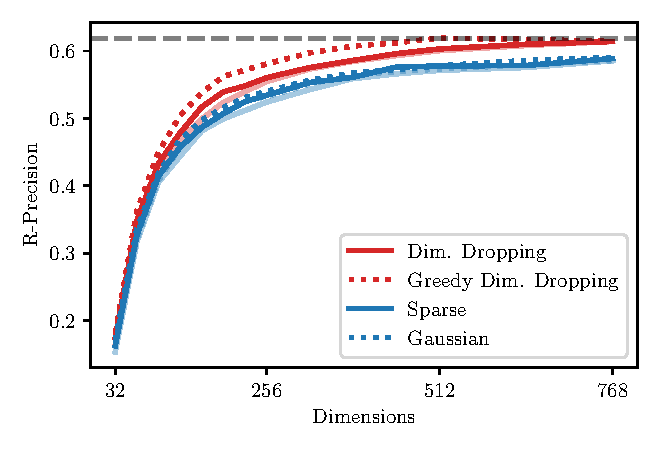
\includegraphics[width=0.7\linewidth]{img/random_projection.pdf}
    
    \caption{Dimension reduction using different random projections methods. Presented values are the max of 3 runs (except for greedy dimension dropping, which is deterministic), semi-transparent lines correspond to the minimum. Embeddings are provided by centered and normalized DPR-CLS. Final vectors are also post-processed by centering and normalization.}
    \label{fig:random_projection}
\end{figure}

\paragraph{Results.}

The results of all random projection methods are shown in \Cref{fig:random_projection}.
Gaussian random projection seems to perform equally to sparse random projection.
The performance is not fully recovered for the two methods.
Interestingly, simply dropping random dimensions led to better performance than that of sparse or Gaussian random projection.
The greedy dimension dropping even improves the performance slightly over random dimension dropping in some cases before saturating and is deterministic.
As shown in \Cref{tab:retrieval_summary}, the greedy dimension dropping with post-processing achieves the best performance among all random projection methods.
Without post-processing, $L_2$ distance works better compared to the inner product. 

\begin{figure*}[ht]
    \center
    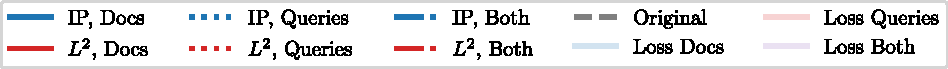
\includegraphics[width=0.85\linewidth]{img/pca_auto_legend.pdf}
    \vspace{0.3cm}

    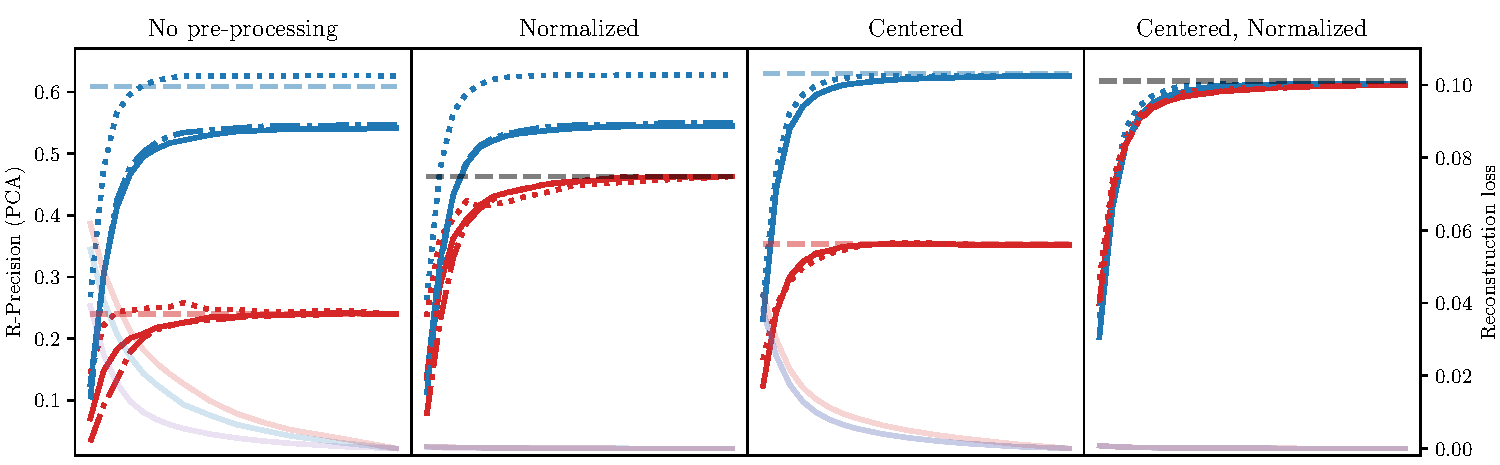
\includegraphics[width=\linewidth]{img/pca_main.pdf}\\
    \vspace{-0.12cm}
    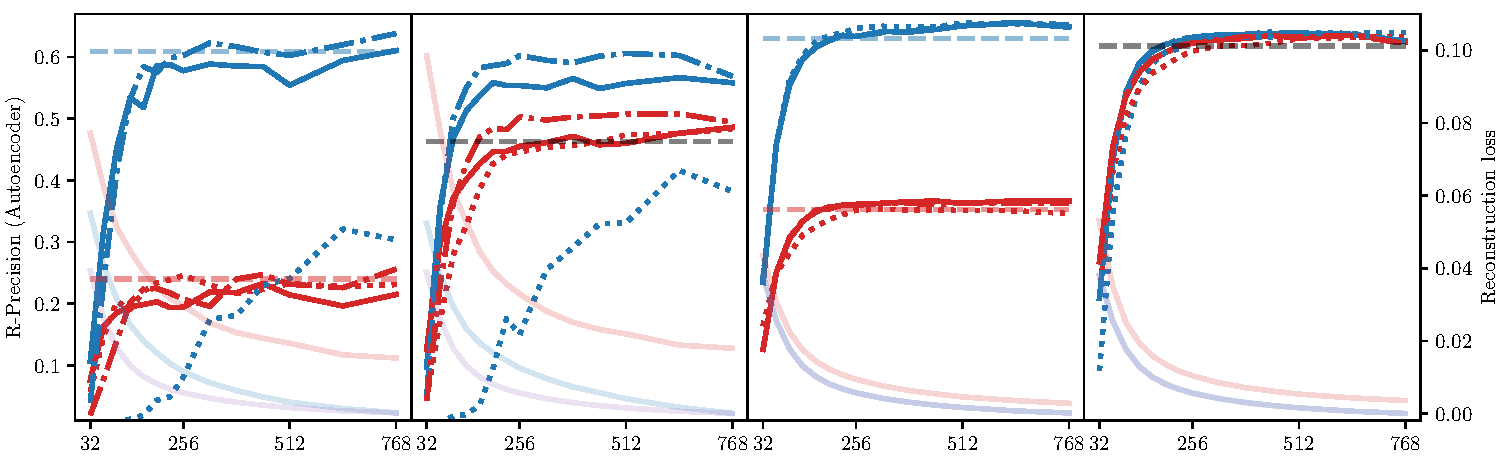
\includegraphics[width=\linewidth]{img/auto_main.pdf}

    \caption{Dimension reduction using PCA (top) and Autoencoder (bottom) trained either on document index, query embeddings or both. Each figure corresponds to one of the four possible combinations of centering and normalizing the input data. The output vectors are not post-processed. Reconstruction loss (MSE, average for both documents and queries) is shown in transparent colour and computed in original data space. Horizontal lines show uncompressed performance. Embeddings are provided by DPR-CLS.}
    \label{fig:pca_auto_main}
\end{figure*}

\subsection{Principal Component Analysis}

Another natural candidate for dimensionality reduction is principal component analysis (PCA) \citep{pca}.
%The usage for dimension reduction was suggested by \citet{izacard2020memory} as one of the possible solutions.
PCA considers the dimensions with the highest variance and omits the rest.
This leads to a projection matrix that projects the original data onto the principal components using an orthonormal basis $T$.
The following loss is minimized $\mathcal{L} = \text{MSE}(\mathbf{T'} \mathbf{T} \bm{x}, \bm{x})$.
Note that we fit PCA on the covariance matrix of either the document index, query embeddings or both and the trained dimension-reducing projection is then applied to both the document and query embeddings.

\paragraph{Results.} The results of performing PCA are shown in \Cref{fig:pca_auto_main}. First, we find that the uncompressed performance, as well as the effect of compression, is highly dependent on the data pre-processing.
This should not be surprising as the PCA algorithm assumes centered and pre-processed data. Nevertheless, we stress and demonstrate the importance of this step.
This is given by the normalization of the input vectors and also that the column vectors of PCA are orthonormal.

Second, when the data is not centered, the PCA is sensitive to what it is trained on.
\Cref{fig:pca_auto_main} show systematically that training on the set of available queries provides better performance than training on the documents or a combination of both. Subsequently, after centering the data, it does not matter anymore what is used for fitting: \textbf{both the queries and the documents provide good estimates of the data variance} and the dependency on training data size for PCA is explored explicitly in \Cref{subsec:model_comparison}.
The reason why queries provide better results without centering is that they are more centered in the first place, as shown in \Cref{tab:dataset_norm}.

\begin{table}[ht]
\center
% values for dpr-c.embd
    \begin{tabular}{lcc}
    \toprule
    & \textbf{Avg.} $\mathbf{L^1}$ \textbf{(std)} & \textbf{Avg.} $\mathbf{L^2}$ \textbf{(std)} \\
    \cmidrule{2-3}
    Documents & $243.0\ (20.1)$ & $12.3\ (0.6)$ \\
    Queries & $137.0\ (7.5)$ & $9.3\ (0.2)$ \\
    \bottomrule
\end{tabular}
\caption{Average $L^1$ and $L^2$ norms of document and query embeddings from DPR-CLS without pre-processing.}
\label{tab:dataset_norm}
\end{table}

In all cases, the PCA performance starts to plateau around $128$ dimensions and is within $95\%$ of the uncompressed performance. 
Finally, we note that while PCA is concerned with minimizing reconstruction loss, \Cref{fig:pca_auto_main}  shows that even after vastly decreasing the reconstruction loss, no significant improvements in retrieval performance are achieved.
We further discuss this finding in \Cref{sec:reconstruction_loss}.

\paragraph{Component Scaling.}
One potential issue of PCA is that there may be dimensions that dominate the vector space.
\citet{mu2017all} suggest to simply remove the dimension corresponding to the highest eigenvalue though we find that simply scaling down the top k eigenvectors systematically outperforms standard PCA.
For simplicity, we focused on the top 5 eigenvectors and performed a small-scale grid-search of the scaling factors.
The best performing one was $(0.5, 0.8, 0.8, 0.9, 0.8)$ and \Cref{tab:retrieval_summary} shows that it provides a small additional boost in retrieval performance.

\subsection{Autoencoder} \label{subsec:auto}

A straightforward extension of PCA for dimensionality reducing is to use autoencoders, which has been widely explored \citep{hu2014improving,wang2016auto}.
Usually, the model is described by an encoder $e : \mathbb{R}^d \rightarrow \mathbb{R}^b$, a function from a higher dimension to the target (bottleneck) dimension and a decoder $r : \mathbb{R}^b \rightarrow \mathbb{R}^d$, which maps back from the target dimension to the original vector space.
The final (reconstruction) loss is then commonly computed as $\mathcal{L} = \text{MSE}((r \circ e)(\bm{x}), \bm{x})$.
To reduce the dimensionality of a dataset, only the function $e$ is applied to both the query and the document embedding.
We consider three models with the bottleneck:
\footnote{$L_b^a$ symbolizes a fully connected linear layer from $a$ dimensions to $b$ dimensions. Layer composition is done with $\circ$.}

\begin{enumerate}
\item A linear projection similar to PCA but without the restriction of orthonormal columns:
\begin{align*}
e_1(\bm{x}) &= L^{768}_{128} \\
r_1(\bm{x}) &= L^{128}_{768}
\end{align*}

\item A multi-layer feed forward neural network with $\tanh$ activation:
\begin{align*}
e_2(\bm{x}) &= L^{768}_{512} \circ \tanh \circ L^{512}_{256} \circ \tanh \circ L^{256}_{128} \\
r_2(\bm{x}) &= L^{128}_{256} \circ \tanh \circ L^{256}_{512} \circ \tanh \circ L^{512}_{768}
\end{align*}

\item The same encoder as in the previous model but with a shallow decoder:
\begin{align*}
e_3(\bm{x}) &= L^{768}_{512} \circ \tanh \circ L^{512}_{256} \circ \tanh \circ L^{256}_{128} \\ r_3(\bm{x}) &= L^{128}_{768}
\end{align*}
\end{enumerate}

Compared to PCA, it is able to model non-pairwise interaction between dimensions (in the case of models 2 and 3 also non-linear interaction).
Hyperparameters are listed in \Cref{tab:auto_config}.

\begin{table}[ht]
\center
\begin{tabular}{ll}
\toprule
\textbf{Hyperparameters} \\ \midrule
Batch size & 128 \\
Optimizer & Adam \\
Learning rate & 10$^{-3}$ \\
$L_1$ regularization & 10$^{-5.9}$ \\
\bottomrule
\end{tabular}
\caption{Hyperparameters of autoencoder architectures.
$L_1$ regularization is used only when explicitly mentioned.}
\label{tab:auto_config}
\end{table}

\paragraph{Results.}
We explore the effects of training data and pre-processing with results for the first model shown in \Cref{fig:pca_auto_main}.
Surprisingly, the Autoencoder is even more sensitive to proper pre-processing than PCA, most importantly centering which makes the results much more stable.

The rationale for the third model is that we would like the hidden representation to require as little post-processing as possible to become the original vector again.
The higher performance of the model with shallow decoder, shown in \Cref{tab:retrieval_summary} supports this reasoning.
An alternative way to reduce the computation (modelling dimension relationships) in the decoder is to regularize the weights in the decoder.
We make use of $L_1$ regularization explicitly because $L_2$ regularization is conceptually already present in Adam's weight decay.
This improves each of the three models.

Similarly to the other reconstruction loss-based method (PCA), without post-processing, the inner product works yields better results.

% I experimented with also one more variation: upscaling with a convolutional kernel (reverse convolution). This made sense because it would force the original dimensions to not be very dependent on each other. Sadly it didn't work much. -Vilém Aug 6, 2021


\begin{table*}[ht]
\center
\renewcommand{\arraystretch}{1.3} % should affect only this table
\resizebox{\linewidth}{!}{%
\begin{tabular}{lccccc}
\toprule
\multirow{2}{*}{\textbf{Method}} & \multirow{2}{*}{\textbf{Compression}} & \multicolumn{2}{c}{\textbf{Original}} & \textbf{Center + Norm.} \\ \cmidrule{3-5}
 &  & IP & $L^2$ & \{IP, $L^2$\} (\% original) \\
\midrule
Original & 1$\times$ & $0.609$ & $0.240$ & ${0.618}\,{\scriptstyle (100\%)}$ \\
\cmidrule{1-5}
Gaussian Projection (128) & 6$\times$ & $0.413$ & $0.453$ & $0.468\,{\scriptstyle (76\%)}$ \\
Sparse Projection (128) & 6$\times$ & $0.398$ & $0.448$& $0.457\,{\scriptstyle (74\%)}$ \\
Dimension Dropping (128) & 6$\times$ & $0.426$ & $0.466$ & $0.478\,{\scriptstyle (77\%)}$  \\
Greedy Dimension Dropping (128) & 6$\times$ & $0.447$ & $0.478$ & ${0.504}\,{\scriptstyle (82\%)}$  \\
\cmidrule{1-5}
PCA (128) & 6$\times$ & $0.577$ & $0.562$ & $0.579\,{\scriptstyle (94\%)}$ \\
PCA (128, scaled top 5) & 6$\times$ & $0.586$ & $0.572$ & ${0.592}\,{\scriptstyle (96\%)}$ \\ % pca/scaled.py
\cmidrule{1-5}
Autoencoder (128, single layer) & 6$\times$ & $0.585$ & $0.569$ & $0.588\,{\scriptstyle (95\%)}$ \\ % --model 1
Autoencoder (128, full) & 6$\times$ & $0.564$ & $0.560$ & $0.588\,{\scriptstyle (95\%)}$ \\ % --model 2
Autoencoder (128, shallow decoder) & 6$\times$ & $0.599$ & $0.582$ & $0.599\,{\scriptstyle (97\%)}$ \\ % --model 3
Autoencoder (128, single layer) + $L_1$ & 6$\times$ & $0.600$ & $0.587$ & ${0.601}\,{\scriptstyle (97\%)}$ \\ % --model 1 --regularize
Autoencoder (128, full) + $L_1$ & 6$\times$ & $0.573$ & $0.569$ & $0.589\,{\scriptstyle (95\%)}$ \\ % --model 2 --regularize
Autoencoder (128, shallow decoder) + $L_1$& 6$\times$ & $0.601$ & $0.591$ & ${0.601}\,{\scriptstyle (97\%)}$ \\ % --model 3 --regularize
\cmidrule{1-5}
Precision 16-bit & 2$\times$ & $0.612$ & $0.610$ & $0.615\,{\scriptstyle (100\%)}$ \\
Precision 8-bit & 4$\times$ & $0.613$ & $0.610$ & $0.614\,{\scriptstyle (99\%)}$ \\
Precision 1-bit (offset $0.5$) & 32$\times$ & $0.559$ & $0.556$ & $0.561\,{\scriptstyle (91\%)}$ \\
Precision 1-bit (offset $0$) & 32$\times$ & $0.530$ & $0.556$ & $0.561\,{\scriptstyle (91\%)}$ \\
\cmidrule{1-5}
PCA (245) + Precision 1-bit (offset $0.5$)  & 100$\times$ & $0.459$ & $0.458$ & ${0.461}\,{\scriptstyle (75\%)}$ \\
PCA (128) + Precision 8-bit & 24$\times$ & $0.558$ & $0.553$ & ${0.567}\,{\scriptstyle (92\%)}$ \\
\bottomrule

% Similarity Distillation $L^2$ & $0.233$  & $0.294$ & $0.285$ \\ % model 4, lr 0.0005
% Similarity Distillation IP & $0.279$  & $0.284$ & $0.XXX$ \\ % model 4, lr 0.0005
% Similarity Distillation $L^2$ + Autoencoder & $0.XXX$ & $0.XXX$ & $0.XXX$ 
% TODO: add delta column to center+norm
% TODO: dont boldface but add subperscript to interesting numbers
\end{tabular}
}
\caption{Overview of compression method performance (from 768) using either $L^2$ or inner product for retrieval. Inputs are based on centered and normalized output of DPR-CLS and the outputs optionally post-processed again. Performance is measured by R-Precision on the pruned HotpotQA dataset.}
\label{tab:retrieval_summary}
\end{table*}


\subsection{Precision Reduction} \label{subsec:prec_reduction}

Lastly, we also experiment with reducing index size by lowering the float precision from 32 bits to 16 and 8 bits.
Note that despite their quite high retrieval performance, they only reduce the size by 2 and 4 respectively (as opposed to 6 by dimension reduction via PCA to 128 dimensions).
Another drawback is that retrieval time is not affected because the dimensionality remains the same.
For more intuition, \Cref{fig:prec_examples,tab:prec_examples} illustrate the effect of floating point precision reduction.
% The 8-bit float is also a non-standard data type not widely supported, therefore the knowledge base would have to be converted to 16-bit floats in the memory nevertheless.

\begin{figure}[ht]
    \center
    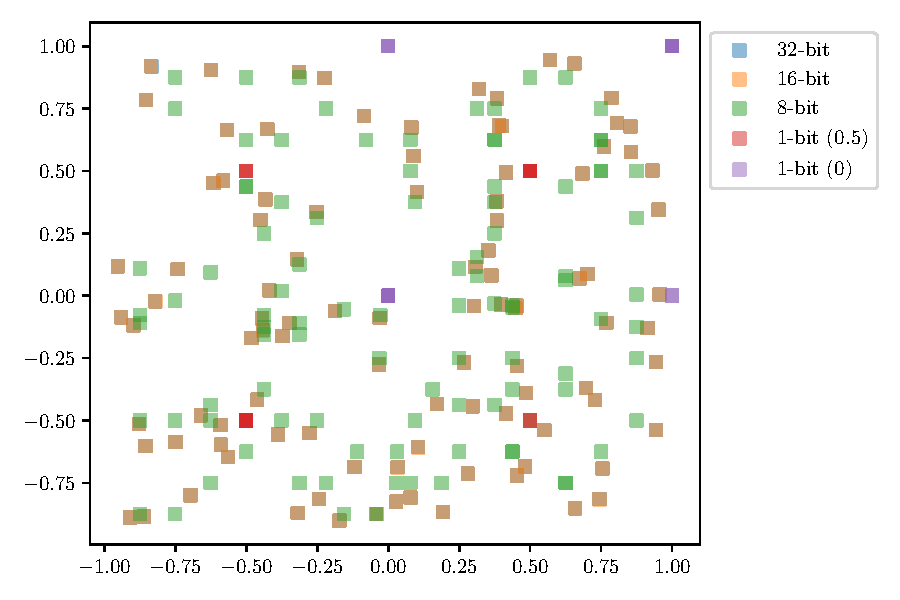
\includegraphics[width=0.85\linewidth]{img/prec_examples.pdf}
    \caption{100 randomly generated points with 5 precision reductions methods. 32-bit and 16-bit overlap, 1-bit has only 4 options.}
    \label{fig:prec_examples}
\end{figure}

\begin{table}[ht]
\center
\begin{tabular}{lllll}
    \toprule
    \hspace{1.3mm}\textbf{32-bit} & \hspace{1.3mm}\textbf{16-bit} & \hspace{1.3mm}\textbf{8-bit} & \hspace{1.3mm}\textbf{1-bit (0.5)} & \textbf{1-bit (0)} \\
    \midrule
    \hspace{1.3mm}0.10159580514915101 & \hspace{1.3mm}0.10162353515625 & \hspace{1.3mm}0.09375 & \hspace{1.3mm}0.5 & 1.0 \\
    \hspace{1.3mm}0.41629564523620965 & \hspace{1.3mm}0.416259765625 & \hspace{1.3mm}0.375 & \hspace{1.3mm}0.5 & 1.0 \\
    -0.41819052217411135 & -0.418212890625 & -0.375 & -0.5 & 0.0 \\
    \hspace{1.3mm}0.02165521039532603 & \hspace{1.3mm}0.0216522216796875\hspace{-5mm} & \hspace{1.3mm}0.01953125 & \hspace{1.3mm}0.5 & 1.0 \\
    \hspace{1.3mm}0.7858939086953094 & \hspace{1.3mm}0.7861328125 & \hspace{1.3mm}0.75 & \hspace{1.3mm}0.5 & 1.0 \\
    \hspace{1.3mm}0.7925861778668761 & \hspace{1.3mm}0.79248046875 & \hspace{1.3mm}0.75 & \hspace{1.3mm}0.5 & 1.0 \\
    -0.7488293790723275 & -0.7490234375 & -0.625 & -0.5 & 0.0 \\
    -0.5855142437236265 & -0.58544921875 & -0.5 & -0.5 & 0.0 \\
    \bottomrule
\end{tabular}
\caption{Decimal representation of randomly generated numbers with 5 precision reduction methods.}
\label{tab:prec_examples}
\end{table}

Using only one bit per dimension is a special case of precision reduction suggested by \citet{yamada2021efficient}.
Because we use centered data, we can define the element-wise transformation function as:
\begin{gather*}
f_\alpha(x_i) = \begin{cases}
1 - \alpha & x_i \ge 0 \\
0 -\alpha & x_i < 0
\end{cases}
\end{gather*}
Bit \texttt{1} would then correspond to $1-\alpha$ and \texttt{0} to $0-\alpha$.
While \citet{yamada2021efficient} use values $1$ and $0$, we work with $0.5$ and $-0.5$ in order to be able to distinguish between certain cases when using IP-based similarity.\footnote{When using $0$ and $1$, the IP similarity of $0$ and $1$ is the same as $0$ and $0$ while for $-0.5$ and $0.5$ they are $-0.25$ and $0.25$ respectively.}
As shown in \Cref{tab:retrieval_summary}, this indeed yields a slight improvement.
When applying post-processing, however, the two approaches are equivalent. While this method achieves extreme 32x compression on the disk and retains most of the retrieval performance.
The downside of 1-bit and 8-bit is that if one wishes to use standard retrieval pipelines, these variables would have to be converted to a supported, larger, data type.

Finally, reducing precision can be readily combined with dimension reduction methods (see \Cref{subsubsec:prec_pca_mult}), such as PCA (prior to changing the data type).
As shown in the last row of \Cref{tab:retrieval_summary}, this can lead to the compressed size be 100x smaller while retaining $75\%$ retrieval performance on HotpotQA and $89\%$ for NaturalQuestions (see \Cref{tab:retrieval_summary_nq}).

\subsection{Combination of PCA and Precision Reduction} \label{subsubsec:prec_pca_mult}

It is possible to combine methods for dimension reduction with methods for reducing data type precision.
The results in \Cref{fig:prec_pca_mult} show that PCA can be combined with e.g. 8-bit precision reduction with negligible loss in performance.

\begin{figure}[ht]
\center
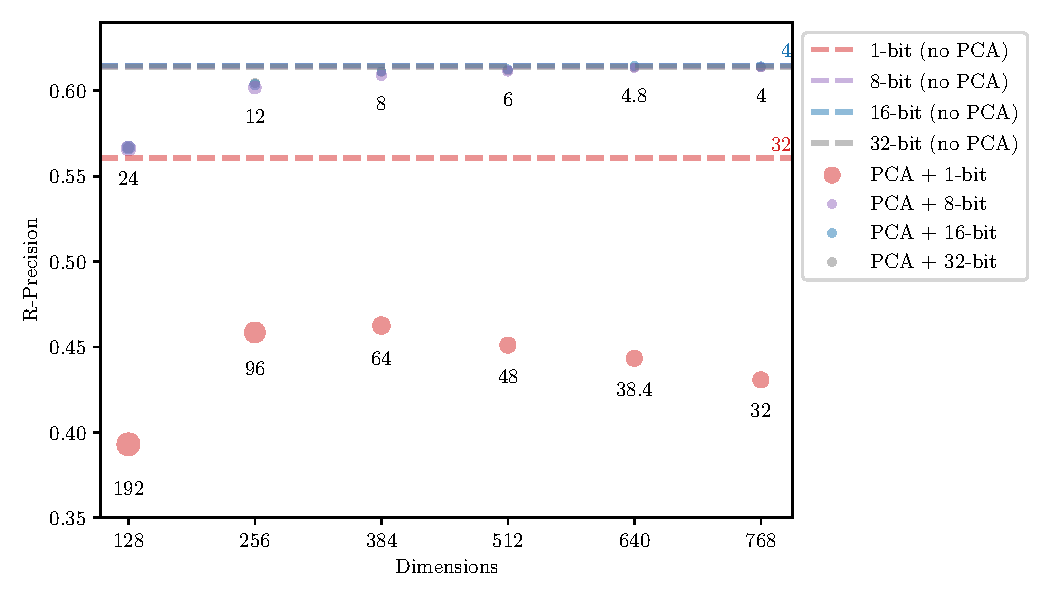
\includegraphics[width=1\linewidth]{img/prec_pca_mult.pdf}
\caption{Combination of PCA and precision reduction. Compression ratio is shown in text.
16-bit and 32-bit values overlap with 8-bit and their compression ratios are not shown. Measured on HotpotQA with DPR-CLS.}
\label{fig:prec_pca_mult}
\end{figure}

\begin{table*}
\center
\renewcommand{\arraystretch}{1.3} % should affect only this table
\resizebox{\linewidth}{!}{%
\begin{tabular}{lcccc}
\toprule
\multirow{2}{*}{\textbf{Method}} & \multirow{2}{*}{\textbf{Compression}} & \multicolumn{2}{c}{\textbf{Original}} & \textbf{Center + Norm.} \\ \cmidrule{3-5}
 &  & IP & $L^2$ & \{IP, $L^2$\} (\% original) \\
\midrule
Original & 1$\times$ & $0.934$ & $0.758$ & $0.920\,{\scriptstyle (100\%)}$ \\
\cmidrule{1-5}
Gaussian Projection & 6$\times$ & $0.825$ & $0.848$ & $0.855\,{\scriptstyle (93\%)}$ \\
Sparse Projection & 6$\times$ & $0.826$ & $0.848$& $0.856\,{\scriptstyle (93\%)}$ \\
Dimension Dropping & 6$\times$ & $0.840$ & $0.863$ & $0.867\,{\scriptstyle (94\%)}$ \\
Greedy Dimension Dropping & 6$\times$ & $0.845$ & $0.873$ & ${0.873}\,{\scriptstyle (95\%)}$  \\
\cmidrule{1-5}
PCA & 6$\times$ & $0.908$ & $0.907$ & $0.910\,{\scriptstyle (99\%)}$ \\
PCA (scaled top 5) & 6$\times$ & $0.916$ & $0.910$ & ${0.920}\,{\scriptstyle (100\%)}$ \\ % pca/scaled.py
\cmidrule{1-5}
Autoencoder (single layer) & 6$\times$ & $0.915$ & $0.910$ & $0.914\,{\scriptstyle (99\%)}$ \\ % --model 1
Autoencoder (full) & 6$\times$ & $0.903$ & $0.907$ & $0.910\,{\scriptstyle (99\%)}$ \\ % --model 2
Autoencoder (shallow decoder) & 6$\times$ & $0.916$ & $0.918$ & $0.919\,{\scriptstyle (100\%)}$ \\ % --model 3
Autoencoder + $L_1$ (single layer) & 6$\times$ & $0.918$ & $0.918$ & ${0.921}\,{\scriptstyle (100\%)}$ \\ % --model 1 --regularize
Autoencoder + $L_1$ (full) & 6$\times$ & $0.909$ & $0.910$ & $0.913\,{\scriptstyle (99\%)}$ \\ % --model 2 --regularize
Autoencoder + $L_1$ (shallow decoder) & 6$\times$ & $0.918$ & $0.917$ & ${0.919}\,{\scriptstyle (100\%)}$ \\ % --model 3 --regularize
\cmidrule{1-5}
Precision 16-bit & 2$\times$ & $0.921$ & $0.917$ & $0.920\,{\scriptstyle (100\%)}$ \\
Precision 8-bit & 4$\times$ & $0.920$ & $0.921$ & $0.922\,{\scriptstyle (100\%)}$ \\
Precision 1-bit (offset $0.5$) & 32$\times$ & $0.902$ & $0.902$ & $0.904\,{\scriptstyle (98\%)}$ \\
Precision 1-bit (offset $0$) & 32$\times$ & $0.892$ & $0.902$ & $0.904\,{\scriptstyle (98\%)}$ \\
\cmidrule{1-5}
PCA (245) + Precision 1-bit (offset $0.5$)  & 100$\times$ & $0.854$ & $0.862$ & ${0.858}\,{\scriptstyle (93\%)}$ \\
PCA (128) + Precision 8-bit & 24$\times$ & $0.906$ & $0.904$ & ${0.909}\,{\scriptstyle (99\%)}$ \\
\bottomrule

% Similarity Distillation $L^2$ & $0.233$  & $0.294$ & $0.285$ \\ % model 4, lr 0.0005
% Similarity Distillation IP & $0.279$  & $0.284$ & $0.XXX$ \\ % model 4, lr 0.0005
% Similarity Distillation $L^2$ + Autoencoder & $0.XXX$ & $0.XXX$ & $0.XXX$ 
\end{tabular}
}
\caption{Overview of compression method performance (from 768) using either $L^2$ or inner product for retrieval. Inputs are based on (1) original and (2) centered and normalized output of DPR-CLS. Performance is measured by R-Precision on NaturalQuestions.}
\label{tab:retrieval_summary_nq}
\end{table*}

\clearpage

\section{Analysis} \label{sec:analysis}

\subsection{Model Comparison} \label{subsec:model_comparison}

The comparison of all discussed dimension reduction methods is shown in \Cref{tab:retrieval_summary}.
It also shows the role of centering and normalization post-encoding which systematically improves the performance.
% Overall, PCA and autoencoder work better than all methods of sparse projections.
The best performing model for dimension reduction is the autoencoder with $L_1$ regularization and either just a single projection layer for the encoder and decoder or with the shallow decoder (6x compression with $97\%$ retrieval performance).

We also show the major experiments in \Cref{tab:retrieval_summary_nq} (table structure equivalent to that for the pruned dataset in \Cref{tab:retrieval_summary}) on Natural Question \citep{kwiatkowski2019natural} with identical dataset pre-processing.
The performance is overall larger because the task is different and the set of documents is lower (1.5 million spans) but comparatively the trends are in line with the previous conclusions of the thesis.

\subsection{Speed.}

Despite the autoencoder providing slightly better retrieval performance and PCA being generally easier to use (due to the lack of hyperparameters), there are several tradeoffs in model selection.
Once the models are trained, the runtime performance (encoding) is comparable though for PCA it is a single matrix projection while for the autoencoder it may be several layers and activation functions.

Depending on the specific library used for implementation, however, the results differ.
\Cref{fig:model_speed} shows that the autoencoder (implemented in PyTorch) is much slower than any other model when run on a CPU but the fastest when run on a GPU.
Similarly, PCA works best if used from the PyTorch library (whether on CPU or GPU) and from the standard Scikit package.
Except for Scikit, there seems to be little relation between the target dimensionality and computation time.

\begin{figure}[ht]
    \center
    % Encoding batch size was 131K
    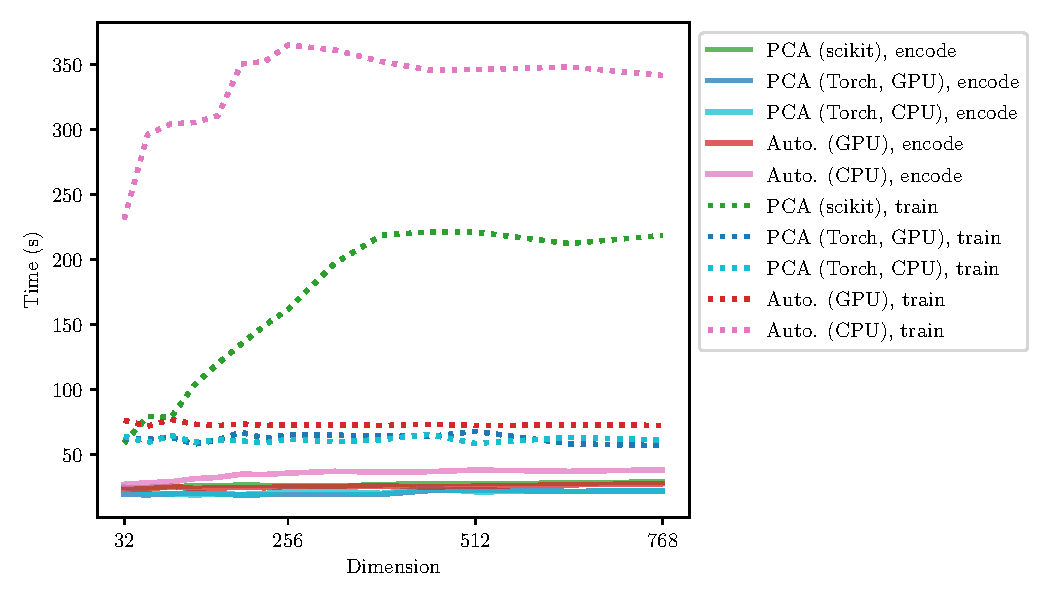
\includegraphics[width=\linewidth]{img/model_speed.pdf}
    \caption{Speed comparison of PCA and autoencoder (model 3) implemented in PyTorch and Scikit\protect\footnotemark split into training and encoding parts. Models were trained on documents and queries jointly (normalized).}
    \label{fig:model_speed}
\end{figure}

\begin{figure}[ht]
% irrelevant_effects.py
    \center
    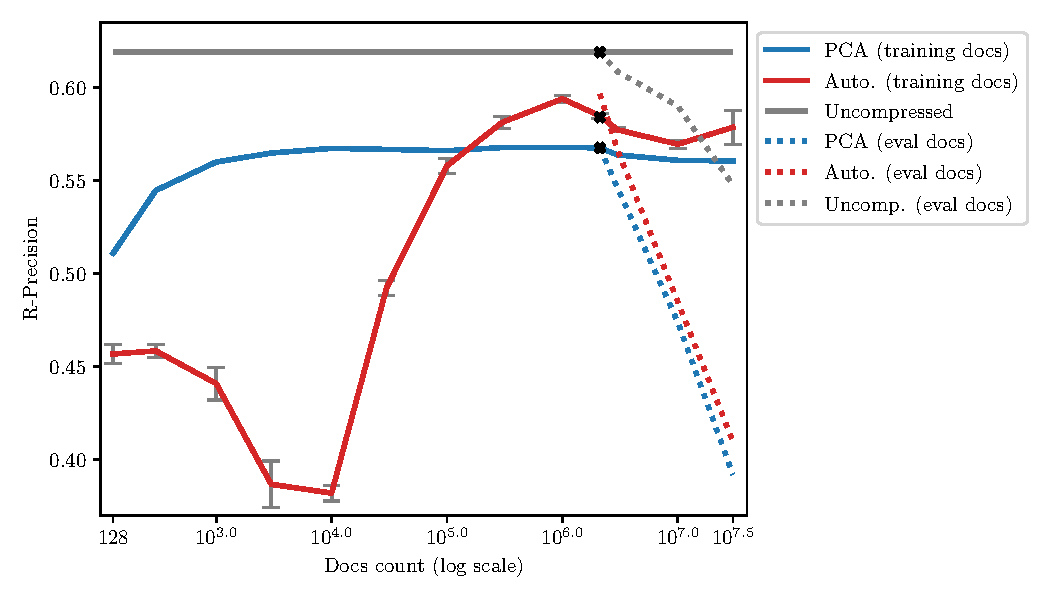
\includegraphics[width=\linewidth]{img/model_data.pdf}

    \captionsetup{type=figure}\caption{Dependency of PCA and autoencoder performance (evaluated on HotpotQA dev data, trained on document encodings) by modifying training data (solid lines) and by adding irrelevant documents to the retrieval pool (dashed lines). Black crosses indicate the original training size. Note the log scale on the x-axis and the truncation of the y-axis.
    }
    \label{fig:model_data}
\end{figure}

\footnotetext{PyTorch 1.9.1, scikit-learn 0.23.2, RTX 2080 Ti (CUDA 11.4), 64$\times$2.1GHz Intel Xeon E5-2683 v4, 1TB RAM.}

% Additionally, \Cref{app_sec:speed} compares training and evaluation speeds of common implementations.

\subsection{Data size}

A crucial aspect of the PCA and autoencoder methods is how much data they need for training.
In the following, we experimented with limiting the number of training samples for PCA and the linear autoencoder.
Results are shown in \Cref{fig:model_data}.


While \citet{ma2021simple} used a much larger training set to fit PCA, we find that PCA requires very few samples (lower-bounded by 128 which is also the number of dimensions used for this experiment).
This is because in the case of PCA training data is used to estimate the data covariance matrix which has been shown to work well when using a few samples \citep{tadjudin1999covariance}.
%to not need much data and new methods for PCA exist \citep{yata2010effective} that require little data.
%Both the PCA and the autoencoder encoder without non-linearity can be represented by a single matrix of the same dimensions, though PCA is further constrained by orthonormality.
Additionally, we find that overall the autoencoder needs more data to outperform PCA.

Next, we experimented with adding more (potentially irrelevant) documents to the knowledge base. %from which to retrieve which were irrelevant and should never be retrieved.
For this, we kept the training data for the autoencoder and PCA to the original size.
The results are shown as dashed lines in \Cref{fig:model_data}.
Retrieval performance quickly deteriorates for both models (faster than for the uncompressed case), highlighting the importance of filtering irrelevant documents from the knowledge base. 

\subsection{Retrieval errors}

So far, our evaluation focused on quantitative comparisons. In the following, we compare the distribution of documents retrieved before and after compression to investigate if there are systematic differences.
We carry out this analysis using HotpotQA which, by design, requires two documents in order to answer a given query.
We compare retrieval with the original document embeddings to retrieval with PCA and 1-bit compression.
%The used datasets Hotpot-QA requires two retrieved documents in order to answer the query.
%We, therefore, examined the distribution of the number of retrieved documents before and after compression to see if there are some systematic shifts.

We find that there are no systematic differences compared to the uncompressed retrieval.
This is demonstrated by the small off-diagonal values in \Cref{fig:hits}.
This result shows that if the retriever working with uncompressed embeddings returns two relevant documents in the top-k for a given query, also the retriever working with the compressed index is very likely to include the same two documents in the top-k.
This is further shown by the Pearson correlation in \Cref{tab:hits_correlation}.
% $\mathlarger{\mathlarger{\rho}}_{\mathcal{D}_\text{dev}} (h_\text{PCA}, h_\text{1-bit})$.

\begin{table}
    \center
    \begin{tabular}{lccc}
        \toprule
        & Uncompressed & PCA & 1bit \\
        \cmidrule{2-4}
        Uncompressed & $1.00$ &  &  \\
        PCA & $0.87$ & $1.00$ &  \\
        1bit & $0.81$ & $0.80$ & $1.00$ \\
        \bottomrule
    \end{tabular}
    \caption{Correlation of the number of retrieved documents for HotpotQA queries in different retrieval modes: uncompressed, PCA (128) and 1-bit precision with R-Precisions (centered \& normalized) of $0.618$, $0.579$ and $0.561$, respectively.}
    \label{tab:hits_correlation}
\end{table}

Overall this suggests that the compressed index can be used on downstream tasks with predictable performance loss based on the slightly worsened retrieval performance.
Furthermore, there do not seem to be any systematic differences even between the two vastly different compression methods used for this experiment (PCA and 1-bit precision).
This indicates that, despite their methodological differences, the two compression approaches seem to remove the same redundances in the uncompressed data.
We leave a more detailed exploration of these findings for future work.

\begin{figure}[ht]
    \center
    
\includegraphics[width=0.02\linewidth]{img/hits_label.pdf}
    \hspace{-0.2cm}
    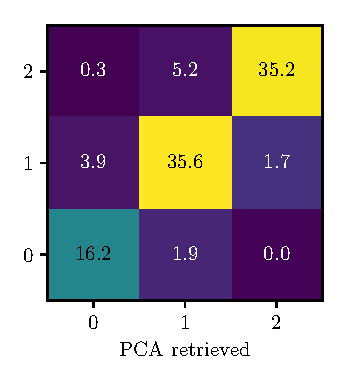
\includegraphics[width=0.35\linewidth]{img/hits_pca.pdf}
    \hspace{-0.39cm}
    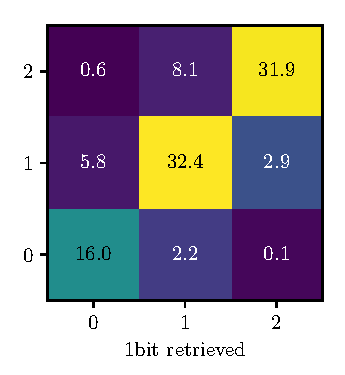
\includegraphics[width=0.35\linewidth]{img/hits_1bit.pdf}
    \caption{Distribution of the number of retrieved documents for HotpotQA queries before and after compression: PCA (128) and 1-bit precision with R-Precisions (centered \& normalized).}
    \label{fig:hits}
\end{figure}

% If configurability is not required and stability or ease of use is desired, PCA is preferred.
% It should be best used from PyTorch regardless of the device.
% If one wishes to have more control of the hyperparameters and wants to utilize the GPU (see \Cref{app_sec:speed}), autoencoder provides slightly better results.
% The whole knowledge base does not need to be used for training compression models, especially for PCA.
% Furthermore, it can be combined with precision reduction.

% \item \textbf{Retrieval errors:} Even vastly different approaches to dimensionality reduction do not systematically retrieve a specific kind of documents. % TODO: rephrase this

% \item Reducing number precision is also a good approach that can be combined with dimension reduction.